\section{Evolu\c{c}\~{a}o microestrutural das amostras T\&P}

\label{sec:micros}

% A evolução microestrutural do material temperado e particionada é avaliada nesta seção de acordo com três variáveis de tratamento térmico. Na seção \ref{sec:micros_tempo} é apresentado o efeito de tempos crescentes de partição na microestrutura do material temperado a \SI{170}{\degreeCelsius} e particionado a \SI{375}{\degreeCelsius}. Na seção \ref{sec:micros_TP} é feita uma avaliação sobre as mudanças microestruturais observadas para diferentes temperaturas de partição. Por fim, na seção \ref{sec:micros_TT} 

% \subsection{Efeito do tempo de partição na microestrutura final}

% \label{sec:micros_tempo}

\subsection{Efeito da temperatura de partição na microestrutura final}

\label{sec:micros_TP}

Nas figuras \ref{fig:TP375MO}a--d são mostradas imagens de microscopia óptica das amostras temperadas a \SI{170}{\degreeCelsius} e particionadas a \SI{375}{\degreeCelsius} por 0, 30~s e, 5~min e 15~min. 
Sob baixa magnificação (200x) podem ser distinguidas regiões escuras, atacadas pelo reagente Nital, e regiões claras, não-atacadas. As regiões não-atacadas correspondem a regiões de MA, isto é, o agregado de austenita retida e martensita formada durante o resfriamento final (martensita fresca, $\alpha'_{fr}$). Antes do resfriamento final as regiões de MA correspondiam a áreas em que a austenita não sofreu transformação durante as etapas do processo T\&P.
Fica claro que as regiões de MA se encontram preferencialmente nas regiões de cotorno de célula. Este comportamento é explicado pelo efeito da microsegregação de elementos de liga na temperatura Ms local, como discutido anteriormente. Com o aumento do tempo de partição, as regiões de contorno de célula, antes ricas em MA, passam a apresentar o padrão de ataque observado no restante da amostra, denotando o consumo da austenita por alguma reação competitiva ao longo da etapa de partição. 

\begin{figure}
  \centering
  \subfloat[]{\includegraphics[width=.48\textwidth]{img/micrografias/170-375/MO/QP0_scalebar.pdf}}
  \quad
  \subfloat[]{\includegraphics[width=.48\textwidth]{img/micrografias/170-375/MO/QP30s_scalebar.pdf}}
  \vspace{0pt}
  \subfloat[]{\includegraphics[width=.48\textwidth]{img/micrografias/170-375/MO/QP5min_scalebar.pdf}}
  \quad
  \subfloat[]{\includegraphics[width=.48\textwidth]{img/micrografias/170-375/MO/QP15min_scalebar.pdf}}
  \caption{}
  % \caption{Amostras T\&P, (a) $T_T$ = \SI{140}{\degreeCelsius}, (b) $T_T$ = \SI{170}{\degreeCelsius}, (c) $T_T$ = \SI{200}{\degreeCelsius}. TP = \SI{300}{\degreeCelsius} / 2h, MEV, aumento de 10kx. Setas azuis indicam placas de martensita e setas vermelhas indicam o produto isotérmico, mais refinado para menores temperaturas de têmpera.}
  \label{fig:TP375MO}
\end{figure}

\begin{figure}
  \centering
  \subfloat[]{\includegraphics[width=.48\textwidth]{img/micrografias/170-375/MO/QP0_1000x_scalebar.pdf}}
  \quad
  \subfloat[]{\includegraphics[width=.48\textwidth]{img/micrografias/170-375/MO/QP30s_1000x_scalebar.pdf}}
  \caption{}
  \label{fig:TP375MO_1000x}
\end{figure}

A identificação microestrutural individual das fases é dificilmente realizada por MO, sendo a microscopia eletrônica de varredura uma técnica mais adequada para este propósito. 
% temperadas a \SI{170}{\degreeCelsius} e particionadas a \SI{375}{\degreeCelsius} por 0, 30~s e, 5~min e 15~min.
As figuras de xx a xx mostram imagens de MEV das mesmas amostras observadas por MO.
Sob o MEV, os aspectos microestruturais identificados incluem placas de martensita ($\alpha'$) atacadas, aquelas formadas durante a etapa de têmpera, com clara presença de carbonetos precipitados internamente. Percebe-que mesmo para o tempo mais curto de partição (0~s, ou seja, temperado imediatamente após a temperatura de partição ser atingida) é observado um relevo na martensita significantemente diferente daquele observado na amostra temperada a \SI{170}{\degreeCelsius}, mas não particionada (Figura \ref{fig:temperaInterrompida}). Um produto acicular, mais fino do que a martensita, é também observado. A fração deste produto aumenta com o tempo de partição. Pela morfologia, é possível identificar com segurança que este microconstituinte consiste de bainita. Para curtos tempos não há evidência de precipitação de carbonetos dentro da bainita, de modo que é também possível inferir que para curtos tempos o produto bainítico consiste apenas de ferrita bainítica ($\alpha_b$), derivada da decomposição incompleta da bainita. Devido ao alto teor de silício e temperatura de transformação, é de fato esperado que um produto bainítico isento de carbonetos seja formado nesta temperatura. 

\begin{figure}
  \centering
  \subfloat[]{\includegraphics[width=.48\textwidth]{img/micrografias/170-375/MEV/0/5kx-3.pdf}}
  \quad
  \subfloat[]{\includegraphics[width=.48\textwidth]{img/micrografias/170-375/MEV/0/20kx-1.pdf}}
  \caption{}
  \label{fig:TP375-0_MEV}
\end{figure}

\begin{figure}
  \centering
  \subfloat[]{\includegraphics[width=.48\textwidth]{img/micrografias/170-375/MEV/30s/5a.pdf}}
  \quad
  \subfloat[]{\includegraphics[width=.48\textwidth]{img/micrografias/170-375/MEV/30s/5b.pdf}}
  \vspace{0pt}
  \subfloat[]{\includegraphics[width=.48\textwidth]{img/micrografias/170-375/MEV/30s/5d.pdf}}
  \quad
  \subfloat[]{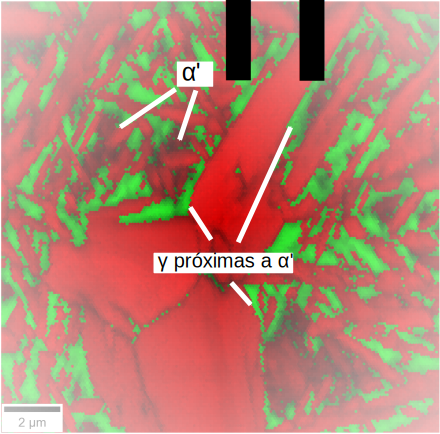
\includegraphics[width=.48\textwidth]{img/micrografias/170-375/MEV/30s/5e.pdf}}
  \caption{}
  \label{fig:TP375-30s_MEV}
\end{figure}

\begin{figure}
  \centering
  \subfloat[]{\includegraphics[width=.48\textwidth]{img/micrografias/170-375/MEV/5min/5kx-6.pdf}}
  \quad
  \subfloat[]{\includegraphics[width=.48\textwidth]{img/micrografias/170-375/MEV/5min/10kx-4.pdf}}
  \caption{}
  \label{fig:TP375-5min_MEV}
\end{figure}

\begin{figure}
  \centering
  \subfloat[]{\includegraphics[width=.48\textwidth]{img/micrografias/170-375/MEV/15min/1300x.pdf}}
  \quad
  \subfloat[]{\includegraphics[width=.48\textwidth]{img/micrografias/170-375/MEV/15min/5kx-8.pdf}}
  \vspace{0pt}
  \subfloat[]{\includegraphics[width=.48\textwidth]{img/micrografias/170-375/MEV/15min/QP170-375-15_phase.pdf}}
  \quad
  \subfloat[]{\includegraphics[width=.48\textwidth]{img/micrografias/170-375/MEV/15min/5f.pdf}}
  \caption{}
  \label{fig:TP375-15min_MEV}
\end{figure}

O microconstituinte MA é observado na imagens de MEV na forma das regiões não atacadas em alto relevo.
Para 30~s um grande bloco de MA é observado em uma região de contorno de célula, com menor fração de martensita primária. Isto reflete a distribuição heterogênea de martensita devido à segregação, como discutido anteriormente. Em regiões com maior fração de $\alpha'$, regiões menores de MA são observados entremeados entre as placas de $\alpha'$ e $\alpha_b$. Ao aumentar o tempo de partição para 15~min não é aparente qualquer variação na fração de fases de carbonetos dentro da martensita. Contudo, é visível que, ao passo que a fração de $\alpha_b$ aumenta, uma pequena fração de carbonetos é formada dentro da bainita, mostrando que o segundo estágio da reação bainítica começara. Como resultado do aumento da fração de $\alpha_b$, a fração e o tamanho dos blocos de MA diminuem, tornando-se mais homogeneamente dispersos na matriz, mesmo nas regiões com menor fração de martensita.
Regiões de MA são observadas para todos os tempos, mesmo para os tempos mais longos, o que não havia sido aparentemente nas observações de MO. É importante salientar que o microconstituinte MA pode ser constituído completamente de austenita retida, de martensita fresca, ou de uma mistura dos dois. No entanto, apenas pela análise de MEV, é impossível determinar com certeza qual é o caso.

% A presença de ferrita bainítica é claramente um elemento importante na microstrutura do ferro fundido T\&P. A fim de comparação, a Figura xx mostra uma imagem de MEV de uma amostra austemperada a \SI{375}{\degreeCelsius} por 15~min, apresentado uma microestrutura de austenita e ferrita bainítica (ou seja, sem martensita primária). É evidente que a estrutura ba

As imagens das condições 30~s e 15~min são acompanhadas dos respectivos mapas de fase obtidos por EBSD (figuras xx e xx). Nos mapas de EBSD, as regiões coloridas em verde representam as fases indexadas com estrutura cúbica de faces centradas (austenita), enquanto as regiões vermelhas correspondem a regiões indexadas como fases cúbicas de corpo centrado (ferrita e martensita). A informação de distribuição de fases é também superposta com a informação de índice de qualidade (IQ) da varredura de EBSD, representada na forma de camada em escala de cinza. Devido às diferenças na concentração de carbono e densidade de discordâncias, os valores de IQ das regiões de $\alpha'_{fr}$ são menores do que nas placas de $\alpha'$, resultando em $\alpha'_{fr}$ aparecendo de forma mais escura do que $\alpha'$. A proporção de $\alpha'_{fr}/\gamma$ nas regiões de MA pode ser observada pela comparação direta dos mapas de fase de EBSD com as imagens de MEV das mesmas regiões. Para 30~s, o grande bloco de MA observado na imagem de MEV é constituído predominantemente de $\alpha'_{fr}$. Por outro lado, os menores blocos de MA constituem-se essencialmente de $\gamma$ retida. É também observado que a maioria da austenita encontrada dentro de blocos de MA está localizada próxima à martensita primária e as placas de ferrita bainítica (figuras xx e xx). Para tempos crescentes a fração de $\alpha'_{fr}$ diminui e a dispersão de $\gamma$ se torna mais homogênea no material.

A estabilização da austenita pelo enriquecimento em carbono é possível por tanto a partição de carbono proveniente da martensita como pela rejeição de carbono durante o crescimento de ferrita bainítica. Em ambos os casos o carbono se acumula na austenita à frente das interfaces e um perfil de carbono transiente é formado. Como consequência, mesmo para curtos tempos de partição a austenita de alto carbono próxima às interfaces é estabilizada durante o resfriamento final. Tal situação é esquematizada na Figura xx. Revertendo o raciocínio, a presença de austenita retira próxima às placas de martensita, tal qual observado na Figura xx, é forte evidência de que a partição de carbono entre martensite e austenita ocorre, mesmo quando carbonetos estão precipitados na martensita.


Imagens de MEV e mapas de fases de EBSD das amostras T\&P particionadas a \SI{300}{\degreeCelsius} e \SI{450}{\degreeCelsius} são mostradas na Figura xx. Com exceção da amostra particionada a \SI{450}{\degreeCelsius}, as microestruturas apresentam detalhes similares àqueles das amostras particionadas a \SI{375}{\degreeCelsius}, sendo compostas primariamente de $\alpha'$, $\alpha_b$ e blocos de MA. A comparação das microestruturas produzidas nas três diferentes temperaturas de partição revela que tanto as estruturas de ferrita bainítica, quanto as dimensões dos carbonetos precipitados na martensita são mais refinados quanto menor a temperatura de partição. 

Notavelmente, para a condição de partição a \SI{450}{\degreeCelsius} por 30~s (Figura xx) é possível observar placas de bainita sendo nucleadas nas interfaces martensita/austenita, sugerindo que a martensita primária desempenha um papel importante assistindo a nucleação bainita. Este fenômeno será discutido em mais detalhes nas próximas seções. Para a condição $T_P = \SI{450}{\degreeCelsius}$ por 15~min, o mapa de fases de EBSD não revela uma fração apreciável de austenita. Imagens de MEV mostram intensa precipitação de carbonetos em ambas martensita e bainita, indicando para esta condição a reação bainítica é completa, tendo consumido toda a austenita.

\subsection{Efeito da temperatura de têmpera na microestrutura final}

\label{sec:micros_TT}

As Figuras \ref{fig:TP300MEV} mostram micrografias obtidas por MEV das microestruturas das amostras temperadas a 140, 170 e \SI{200}{\degreeCelsius} e em seguida particionadas a \SI{300}{\degreeCelsius} por 15 minutos. Na análise dos resultados apresentados adiante, a temperatura de partição foi mantida fixa para que a morfologia do produto isotérmico formado durante a partição fosse a mesma para as amostras avaliadas, de modo a levar em conta apenas a influência da temperatura de têmpera. Por sua vez, o principal efeito da temperatura de têmpera na evolução microestrutural é o controle da quantidade inicial de martensita e, consequentemente, a quantidade inicial de austenita não-transformada.

Embora os resultados de dilatometria apontem a existência de maiores quantidades de placas martensita na amostra temperada a \SI{140}{\degreeCelsius} (Figura \ref{fig:TP300MEV}a), essa diferença é pouco perceptível na análise microestrutural. Por outro lado, nota-se uma nítida diferença na dimensão longitudinal dos feixes do produto bainítico. A ferrita bainítica formada após têmpera a \SI{200}{\degreeCelsius} parece ser consideravelmente mais alongada do que aquela formada após têmpera a \SI{170}{\degreeCelsius}, que por sua vez é mais alongada do que a formada após a têmpera a \SI{140}{\degreeCelsius}. Isto é, quanto menor a temperatura de têmpera --- ou seja, quanto maior a quantidade inicial de martensita formada durante a têmpera --- mais refinado é o produto bainítico.

%As Figuras \ref{fig:TT140TP300}a e \ref{fig:TT140TP300}b mostram a microestrutura da amostra temperada a \SI{140}{\degreeCelsius} e particionada a \SI{300}{\degreeCelsius}. Em baixo aumento (100x) é possível observar extensas áreas brancas, associadas a regiões com maior predominância de austenita retida. Por sua vez, a localização da austenita é relacionada aos contornos de célula eutética formados durante a solidificação. Devido à segregação de elementos durante a solidificação do metal para estas regiões, espera-se que uma quantidade maior de austenita retida seja observada nesses locais. Esse mesmo comportamento é observados nas demais amostras tratadas termicamente.

%\begin{figure}
  %\centering
  %\subfloat[]{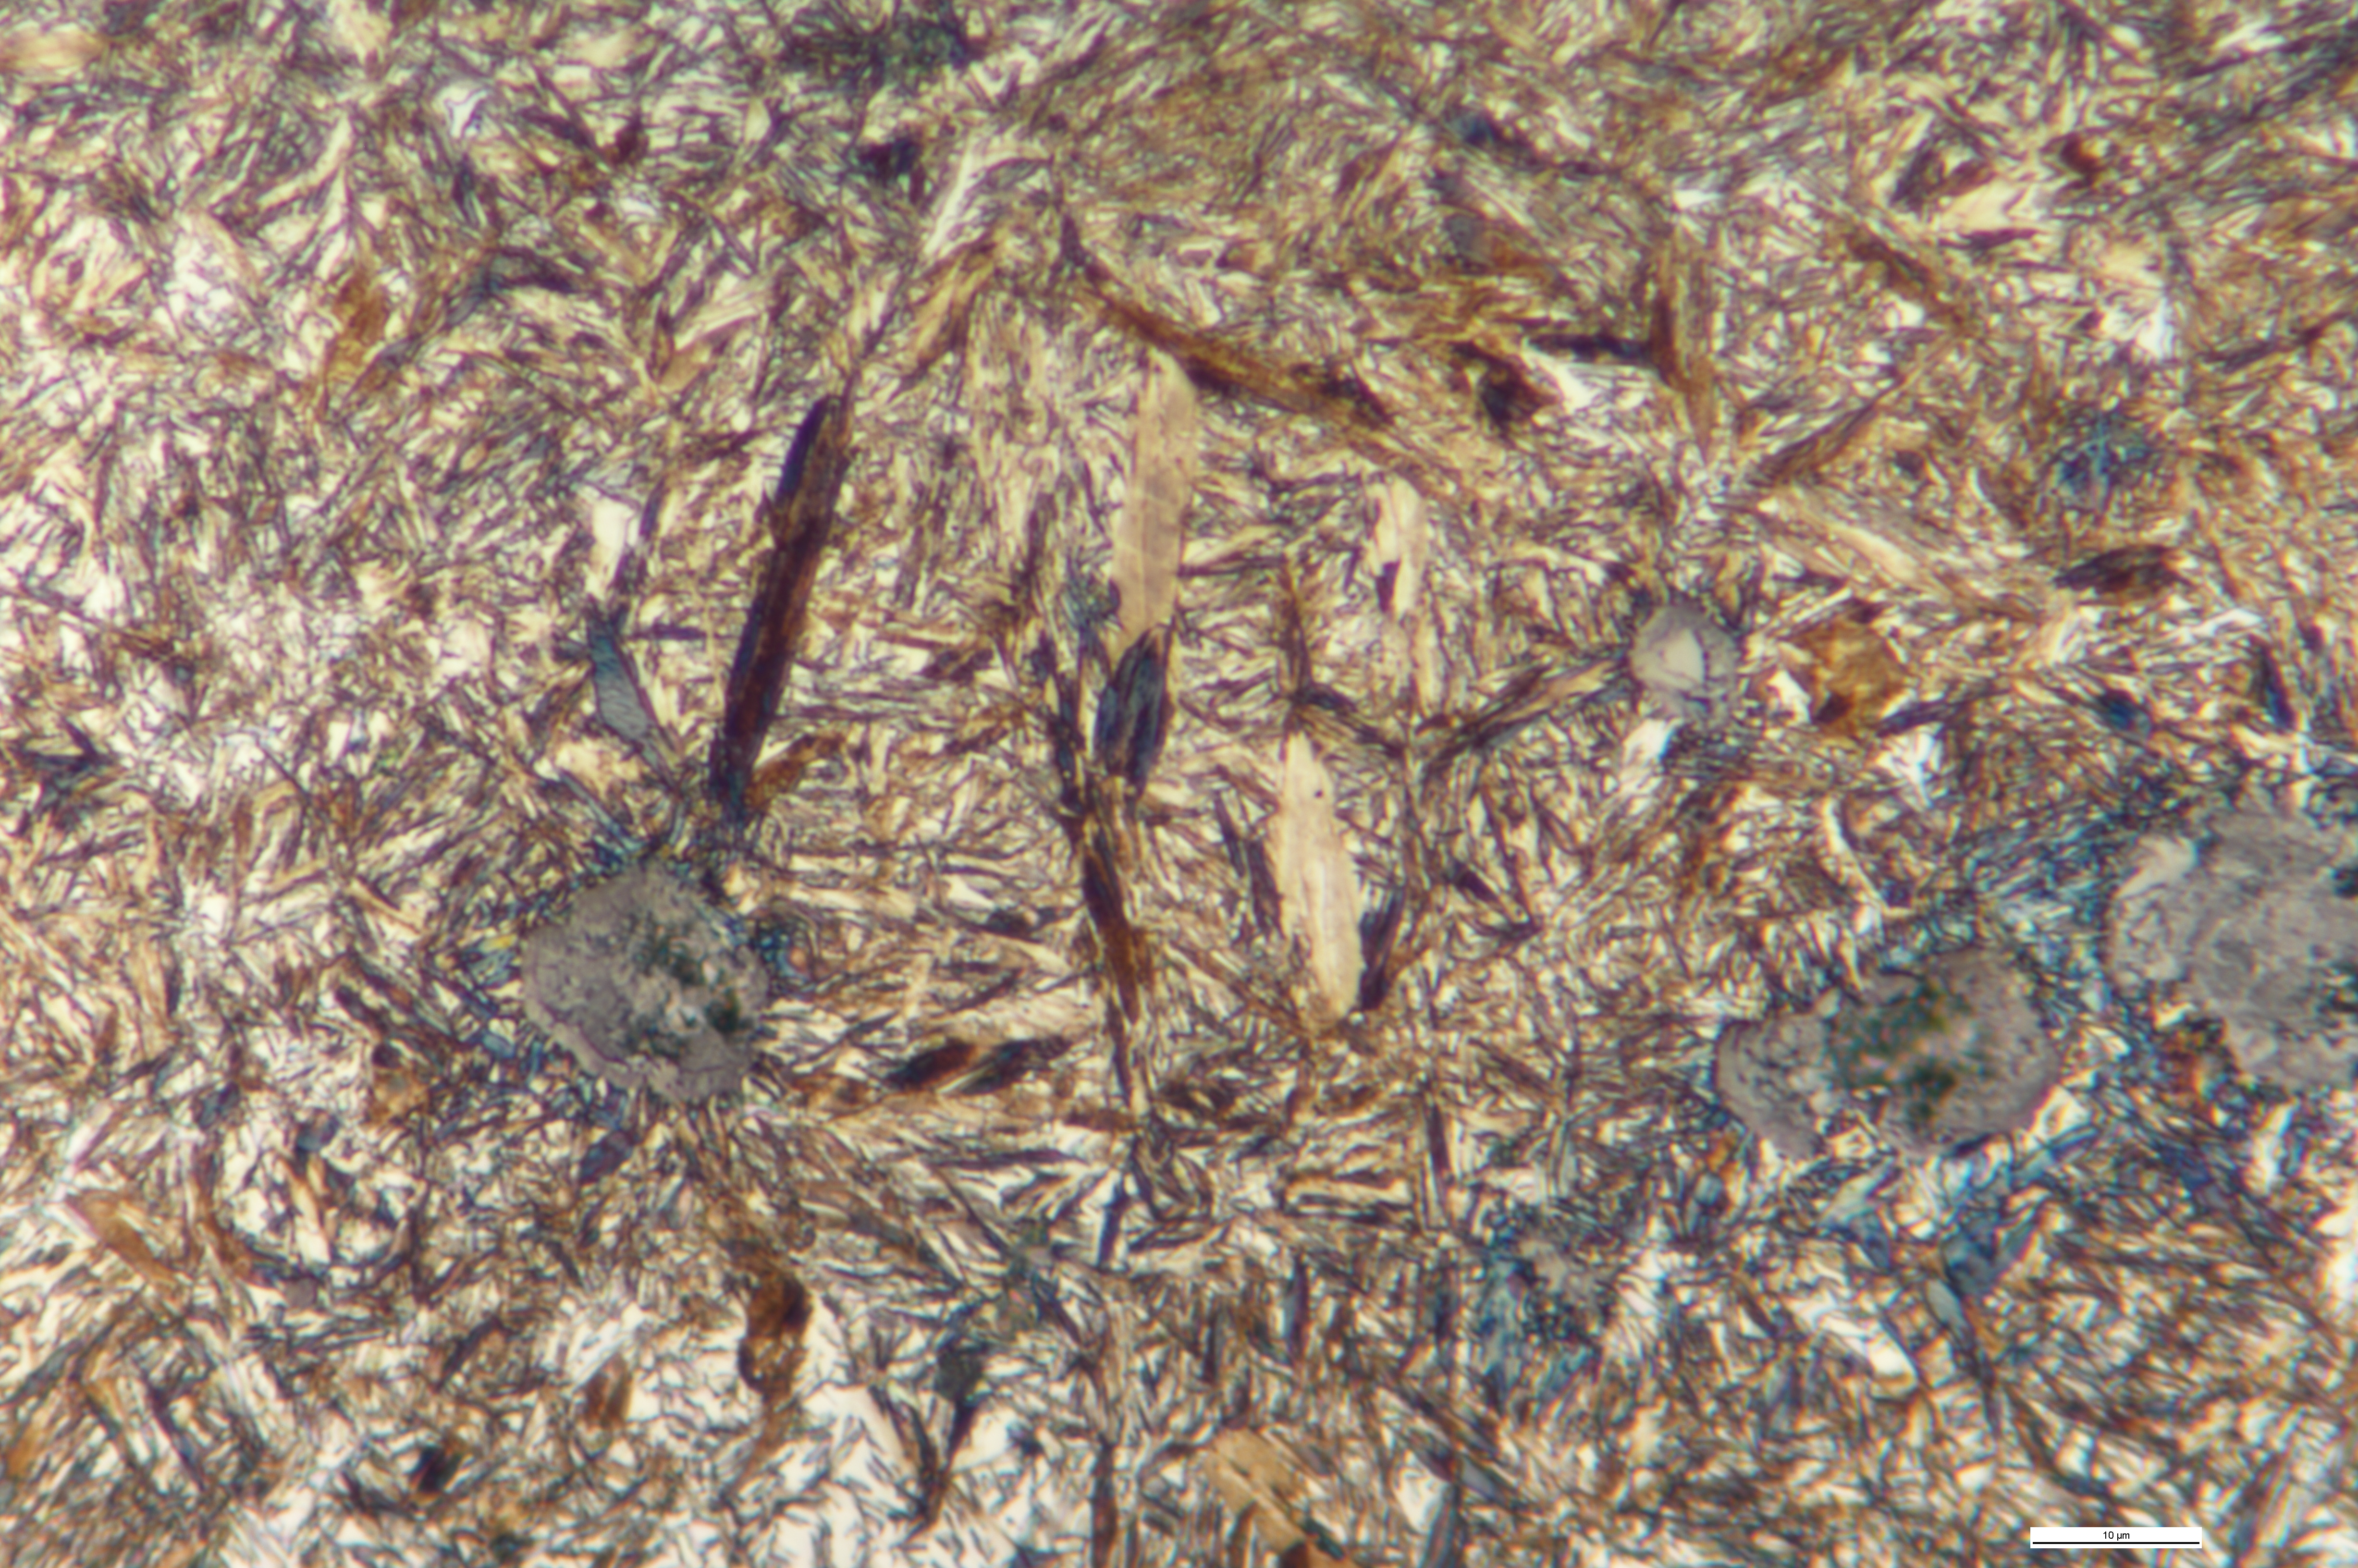
\includegraphics[width=.48\textwidth]{img/micrografias/MO/TT140TP300/1000x-1.pdf}}
  %\quad
  %\subfloat[]{\includegraphics[width=.48\textwidth]{img/micrografias/MO/TT170TP300/1000x-2.pdf}}
  %\vspace{0pt}
  %\subfloat[]{\includegraphics[width=.48\textwidth]{img/micrografias/MO/TT200TP300/1000x-2.pdf}}
  %\caption{Imagens obtidas por microscopia óptica da amostra temperada a \SI{140}{\degreeCelsius} e particionada a \SI{300}{\degreeCelsius}. (a) Aumento de 100x. (b) Aumento de 1000x.}
  %\label{fig:TP300MO}
%\end{figure}

\begin{figure}
  \centering
  \subfloat[]{\includegraphics[width=.48\textwidth]{img/micrografias/efeito_tempera/TT140TP300/10k-4.pdf}}
  \quad
  \subfloat[]{\includegraphics[width=.48\textwidth]{img/micrografias/efeito_tempera/TT170TP300/10k-1.pdf}}
  \vspace{0pt}
  \subfloat[]{\includegraphics[width=.48\textwidth]{img/micrografias/efeito_tempera/TT200TP300/10k-1.pdf}}
  \caption{Amostras T\&P, (a) $T_T$ = \SI{140}{\degreeCelsius}, (b) $T_T$ = \SI{170}{\degreeCelsius}, (c) $T_T$ = \SI{200}{\degreeCelsius}. TP = \SI{300}{\degreeCelsius} / 2h, MEV, aumento de 10kx. Setas azuis indicam placas de martensita e setas vermelhas indicam o produto isotérmico, mais refinado para menores temperaturas de têmpera.}
  \label{fig:TP300MEV}
\end{figure}

Este resultado pode ser explicado pela repartição dos grãos originais de austenita pela martensita. Quanto maior a quantidade inicial de martensita (temperaturas de têmpera mais elevadas), menor o tamanho de grão da austenita não transformada. Logo, uma vez que o crescimento dos feixes de bainita é limitado pelos contorno de grão --- sejam entre dois grãos de austenita, seja entre uma placa de martensita [ou outro feixe de bainita] e a austenita --- menor a dimensão do produto bainítico formado.

Isso fica ainda mais claro quando as microestruturas das amostras T\&P é comparada com a microestrutura do material submetido ao tratamento de austêmpera (ADI), mostrada na Figura \ref{fig:ADI300MEV}. Note-se que, enquanto os feixes de ferrita bainítica na amostra temperada a \SI{140}{\degreeCelsius} e particionada a \SI{300}{\degreeCelsius} possuem cerca de \SI{5}{\mu m} de comprimento, o feixe de bainita no ADI produzido após austêmpera a \SI{300}{\degreeCelsius} por 15 minutos (Figura \ref{fig:ADI300MEV}) possui aproximadamente \SI{20}{\mu m} de comprimento.

\begin{figure}
  \centering
  \subfloat[]{\includegraphics[width=.48\textwidth]{img/micrografias/efeito_tempera/ADI300/2500x-1.pdf}}
  \quad
  \subfloat[]{\includegraphics[width=.48\textwidth]{img/micrografias/efeito_tempera/ADI300/10k-1.pdf}}
  \caption{Amostra austemperada a \SI{300}{\degreeCelsius} / 15 minutos. (a) MEV, 2500x. (b) MEV, 10kx. Nota-se que a bainita é ainda mais alongada do que nas amostras T\&P. É possível também ver detalhes da subestrutura dos feixes de bainita, como subunidades e filmes de austenita entre ripas.}
  \label{fig:ADI300MEV}
\end{figure}
